\documentclass{article}
\setlength\parindent{24pt}
\usepackage[margin=0.6in]{geometry}
\usepackage{indentfirst}
\usepackage{amsmath}
\usepackage{graphicx}
\usepackage{float}
\usepackage[utf8]{inputenc}
\usepackage{listings}
\usepackage{color}
\usepackage{enumerate}
\usepackage[portuguese]{babel}

\definecolor{dkgreen}{rgb}{0,0.6,0}
\definecolor{gray}{rgb}{0.5,0.5,0.5}
\definecolor{mauve}{rgb}{0.58,0,0.82}

\lstset{frame=tb,
  language=Matlab,
  aboveskip=3mm,
  belowskip=3mm,
  showstringspaces=false,
  columns=flexible,
  basicstyle={\small\ttfamily},
  numbers=none,
  numberstyle=\tiny\color{gray},
  keywordstyle=\color{blue},
  commentstyle=\color{dkgreen},
  stringstyle=\color{mauve},
  breaklines=true,
  breakatwhitespace=true,
  tabsize=4
}

\renewcommand{\baselinestretch}{1.0}

\begin{document}

\title{EA614 - Análise de Sinais \\
\large{EFC6 - Transformada Discreta de Fourier}}
\author{Rafael Gonçalves (186062)}
\date{\today}

\maketitle

\begin{enumerate}[(a)]
\item

    Gráfico de $x[n]$:

\begin{figure}[H]
\centering
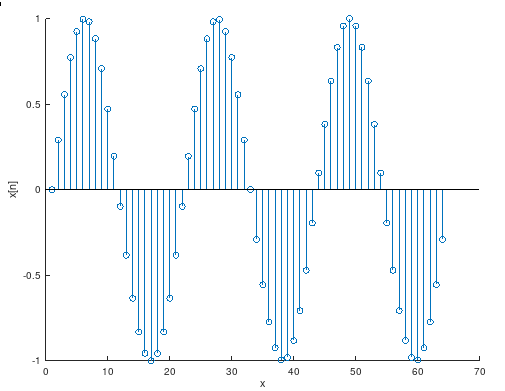
\includegraphics[width=0.5\textwidth]{images/xn.png}
    \caption{$x[n]$ por $n$ com $N = 64$}
\end{figure}

\item

    \[
    X(e^{j\Omega}) = \sum\limits_{n = -\infty}^{\infty} x[n] e^{-j\Omega n}
\]

        \[
    x[n] = \sin(2\pi\frac{f_0}{f_s}n)w_N[n] \quad  N = 64,  f_0 = 3,  f_s = 64
\]

        \[
    X(e^{j\Omega}) = \sum\limits_{n = 0}^{63} \sin(2\pi\frac{3}{64}n) e^{-j\Omega n}
\]

        \[
            \Omega_0 = 2 \pi \frac{ f_0 }{f_s} \quad\quad
            \Omega = 2 \pi \frac{ f }{f_s}
        \]

        \[
            X(e^{j\Omega}) = \sum\limits_{n = 0}^{63} \frac{1}{2j}[e^{j \Omega_0 n} - e^{-j \Omega_0 n}] e^{-j\Omega n} = \sum\limits_{n = 0}^{63} \frac{1}{2j}[e^{-j (\Omega + \Omega_0)  n } - e^{-j (\Omega - \Omega_0) n}]
        \]

        Pela fórmula de soma de PGs finitas temos:

        \[
            \boxed{
            X(e^{j\Omega}) = \frac{1}{2j}\left [ \left ( \frac{1 - e^{63(\Omega - \Omega_0)}}{1 - e^{(\Omega - \Omega_0)}} \right ) - \left ( \frac{1 - e^{63(\Omega + \Omega_0)}}{1 - e^{(\Omega + \Omega_0)}} \right ) \right ]
            }
        \]

\item

    Gráfico de $X[k]$ e $X(e^{j\Omega})$ entre $0$ e $\pi$:

\begin{figure}[H]
\centering
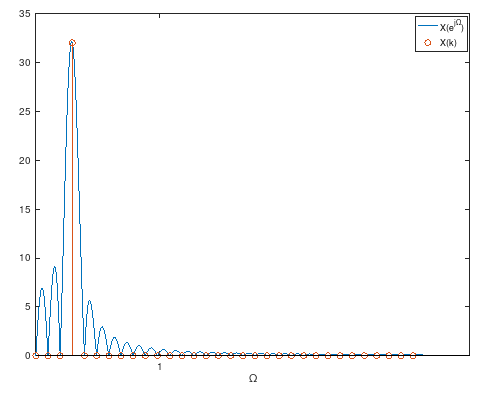
\includegraphics[width=0.5\textwidth]{images/xk_xejomega.png}
    \caption{$X[k]$ e $X(e^{j\Omega})$ em função de $\Omega$}
\end{figure}

\item

    $X[k]$ representa o mesmo sinal $X(e^{j\Omega})$ amostrado em N pontos igualmente espaçados entre todo o espectro que não se repete (ou seja, N pontos entre $\Omega = 0$ até $\Omega = 2\pi$). No caso específico do plot acima, a amostragem coincidiu com o ponto de frequência mais expressivo de $X(e^{j\Omega})$ sendo nulo nos outros pontos. Portanto o sinal $X[k]$ representa bem o sinal original da senóide pura.

\item

Gráficos com $f_0 = 3.4$ Hz:

\begin{figure}[H]
\centering
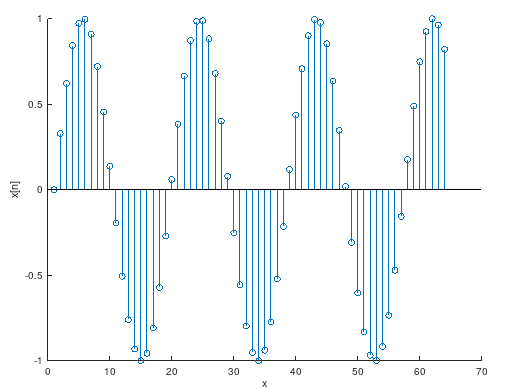
\includegraphics[width=0.5\textwidth]{images/xn_3-4.png}
    \caption{$x[n]$ por $n$ com $N = 64$}
\end{figure}

\begin{figure}[H]
\centering
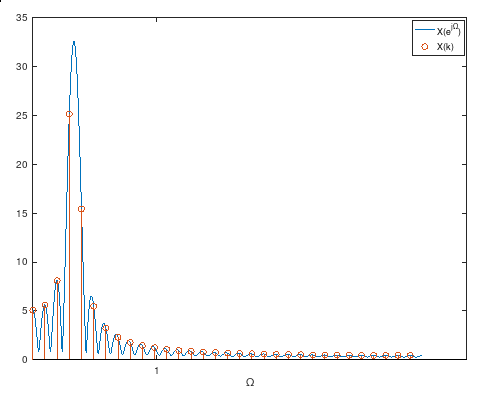
\includegraphics[width=0.5\textwidth]{images/xk_xejomega_3-4.png}
    \caption{$X[k]$ e $X(e^{j\Omega})$ em função de $\Omega$}
\end{figure}

O espectro $X[k]$ obtido não representa bem uma senóide pura. A senóide pura deveria ter seu sinal no domínio da frequência representado por um único ponto não nulo (entre $0$ e $\pi$) para a variável $k$. O vazamento de frequências (frequências não nulas em outros pontos do eixo $k$ - ou neste caso no eixo $\Omega$) ocorre pois a taxa de amostragem escolhida para a DFT (N = 64) não é adequada para representar o sinal. O sinal recuperado no eixo do tempo (após a DFT inversa) terá deformações (aliasing) fruto dessas frequências indesejadas.


\end{enumerate}
\end{document}
